\input{../../Headers/ExerciseswNotesH} % ExercisesH, ExerciseswNotesH, ExercisesHandoutH, NotesH
% (= SlidesH, SlideswNotesH, HandoutH, NotesH, Slides2ScreensH,

\graphicspath{{../../../images/Exercises/}} % Location of the slide background and figure files

%----------------------------------------------------------------------------------------
%	TITLE PAGE
%----------------------------------------------------------------------------------------

\title{Handstand and preliminary exercises} % The short title appears at the bottom of every slide, the full title is only on the title page

\documentclass[../main.tex]{subfiles}
\graphicspath{{\subfix{../images/}}}
\begin{document}

\author{Raphael Nussbaum} % Your name
\institute[Stress Regulation] % Your institution as it will appear on the bottom of every slide, may be shorthand to save space
{
AJ Tutoring Nerd Fest \\
%Stress regulation YouTube channel \\ % Your institution for the title page
\medskip
\textit{raphaelnussbaum@ajtutoring.com}
%regulate.stress@gmail.com} % Your email address
}
\date{\today} % Date, can be changed to a custom date

\end{document}

\begin{document}

\begin{frame}
\titlepage % Print the title page as the first slide
\end{frame}



%-------------------------------------------------------------------
\begin{frame}
\frametitle{Starting position}
\hypertarget{hemi}{}
\begin{columns}[c] % The "c" option specifies centered vertical alignment while the "t" option is used for top vertical alignment

\column{0.7\textwidth} % Left column and width
%	\begin{figure}
	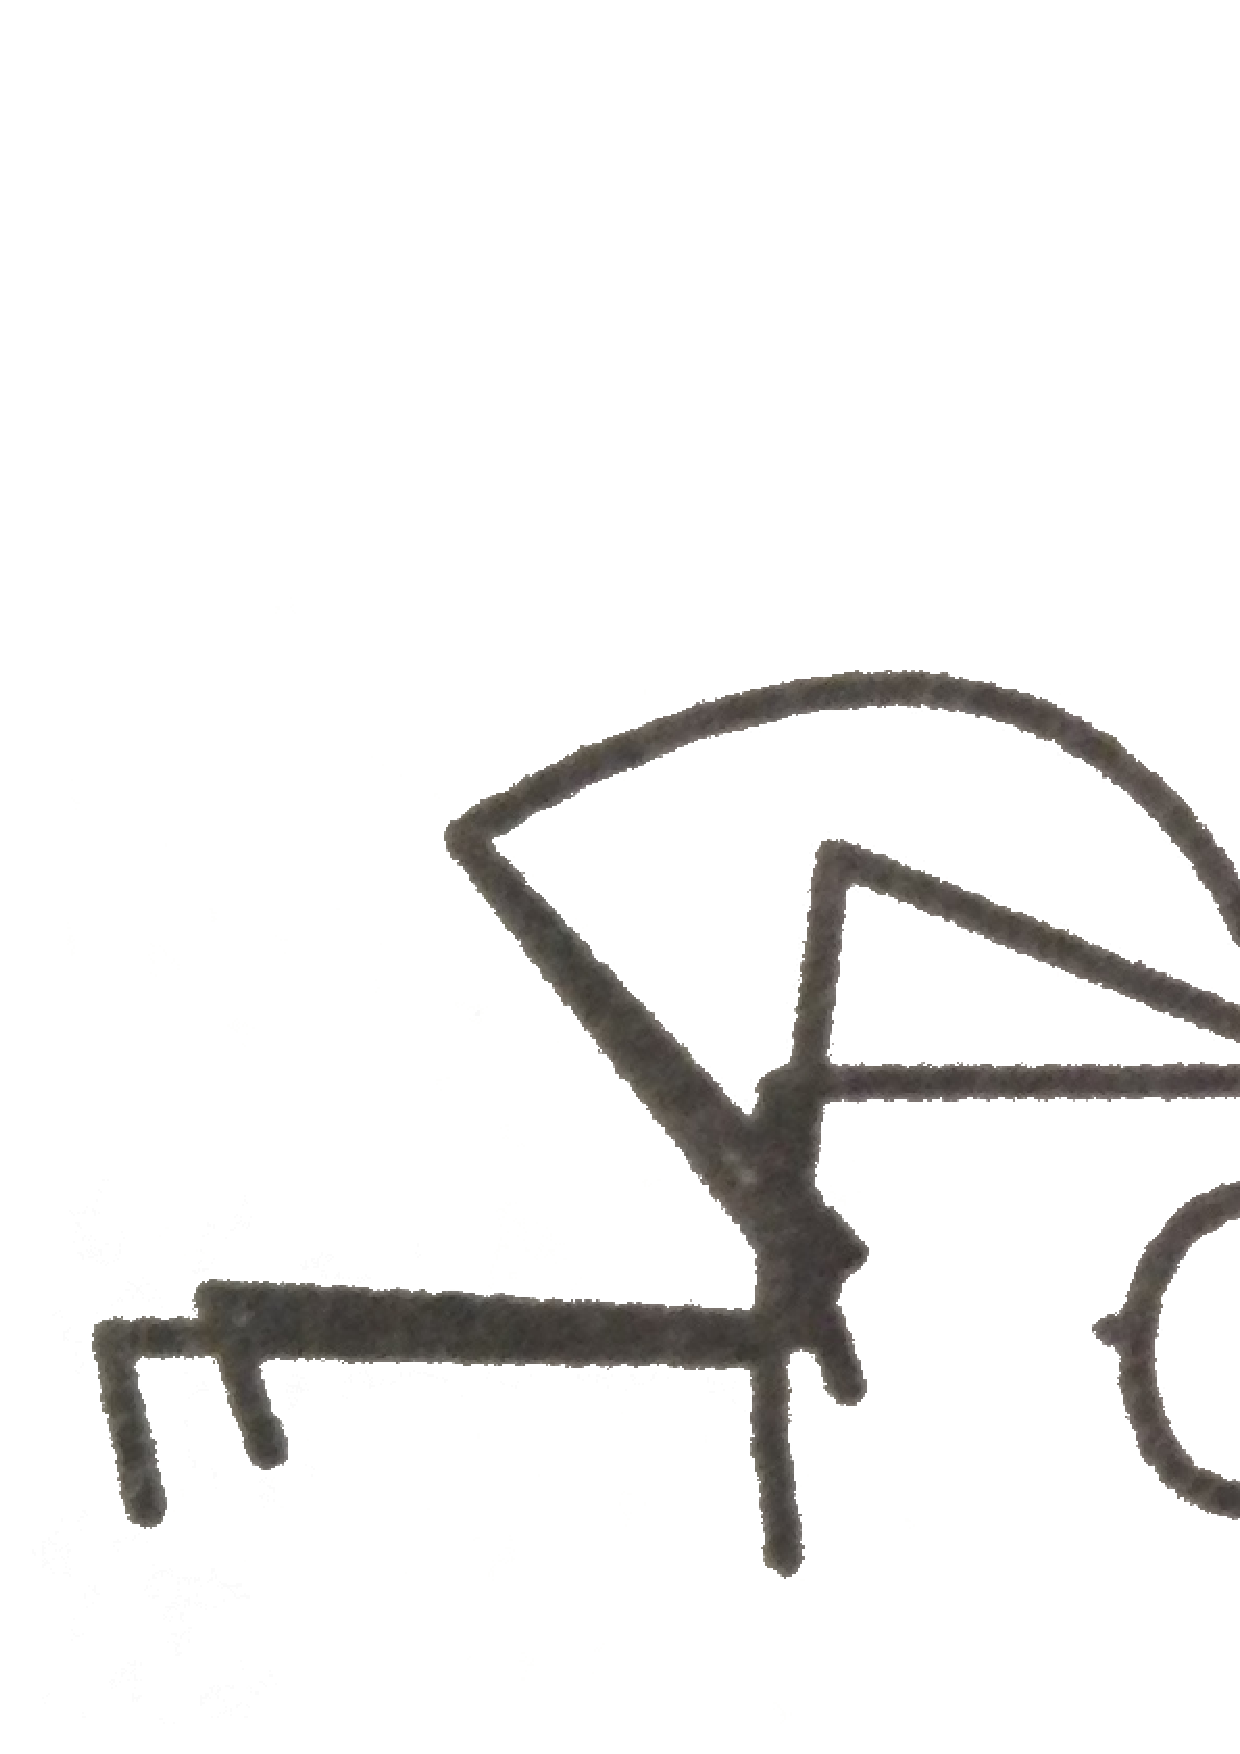
\includegraphics[width=1\linewidth]{HS_position.png}
%	\end{figure}

	\column{0.4\textwidth} % Left column and width
\structure{Kneel} down with your toes  tucked in and make a \structure{triangle with your hands and the head}, which is put on the ground with the crown, the highest point, touching the ground.                    

\structure{Roll your head gently} back and forwards.                                                                                                                                                                                                                                                                                                                                                                                                                                                                                                                                                                                                                                                                                                                                                                                                                                                                                                                                                                                                                                                                                                                                                                                                                                                                                                                                                                                                                                                                                                                                                                                                                                                                                                                                                                                                                                                                                                                                                                                                                                                                                                                                                                                                                                                                                                                                                                                                                                                                                                                                                                                                                                                                                                                                                                                                                                                                                                                                                                                                                                                                                                                                                                                                                                                                                                                                                                                                                                                                                                                                                                                                                                                                                                                                                                                                                                                                                                                                                                                                                                                                                                                                                                                                                                                                                                                                                                                                                                                                                                                                                                                                                                                                                                                                                                                                                                                                                                                                                                                                                                                                                                                                                                                                                                                                                                                                                                                                                                                                                                                                                                                                                                                                                                                                                                                                                                                                                                                                                                                                                                                                                                                                                                                                                                                                                                                                                                                                                                                                                                                                                                                                                                                                                                                                                                                                                                                                                                                                                                                                                                                                                                                                                                                                                                                                                                                                                                                                                                                                                                                                                                                                                                                                                                                                                                                                                                                                                                                                                                                                                                                                                                                                                                                                                                                                           
\end{columns}
\end{frame}
%---------------------------------------------------------------------------------

%-------------------------------------------------------------------
\begin{frame}
\frametitle{Shifting your weight}
\hypertarget{hemi}{}
\begin{columns}[c] % The "c" option specifies centered vertical alignment while the "t" option is used for top vertical alignment

\column{0.22\textwidth} % Left column and width
%	\begin{figure}
	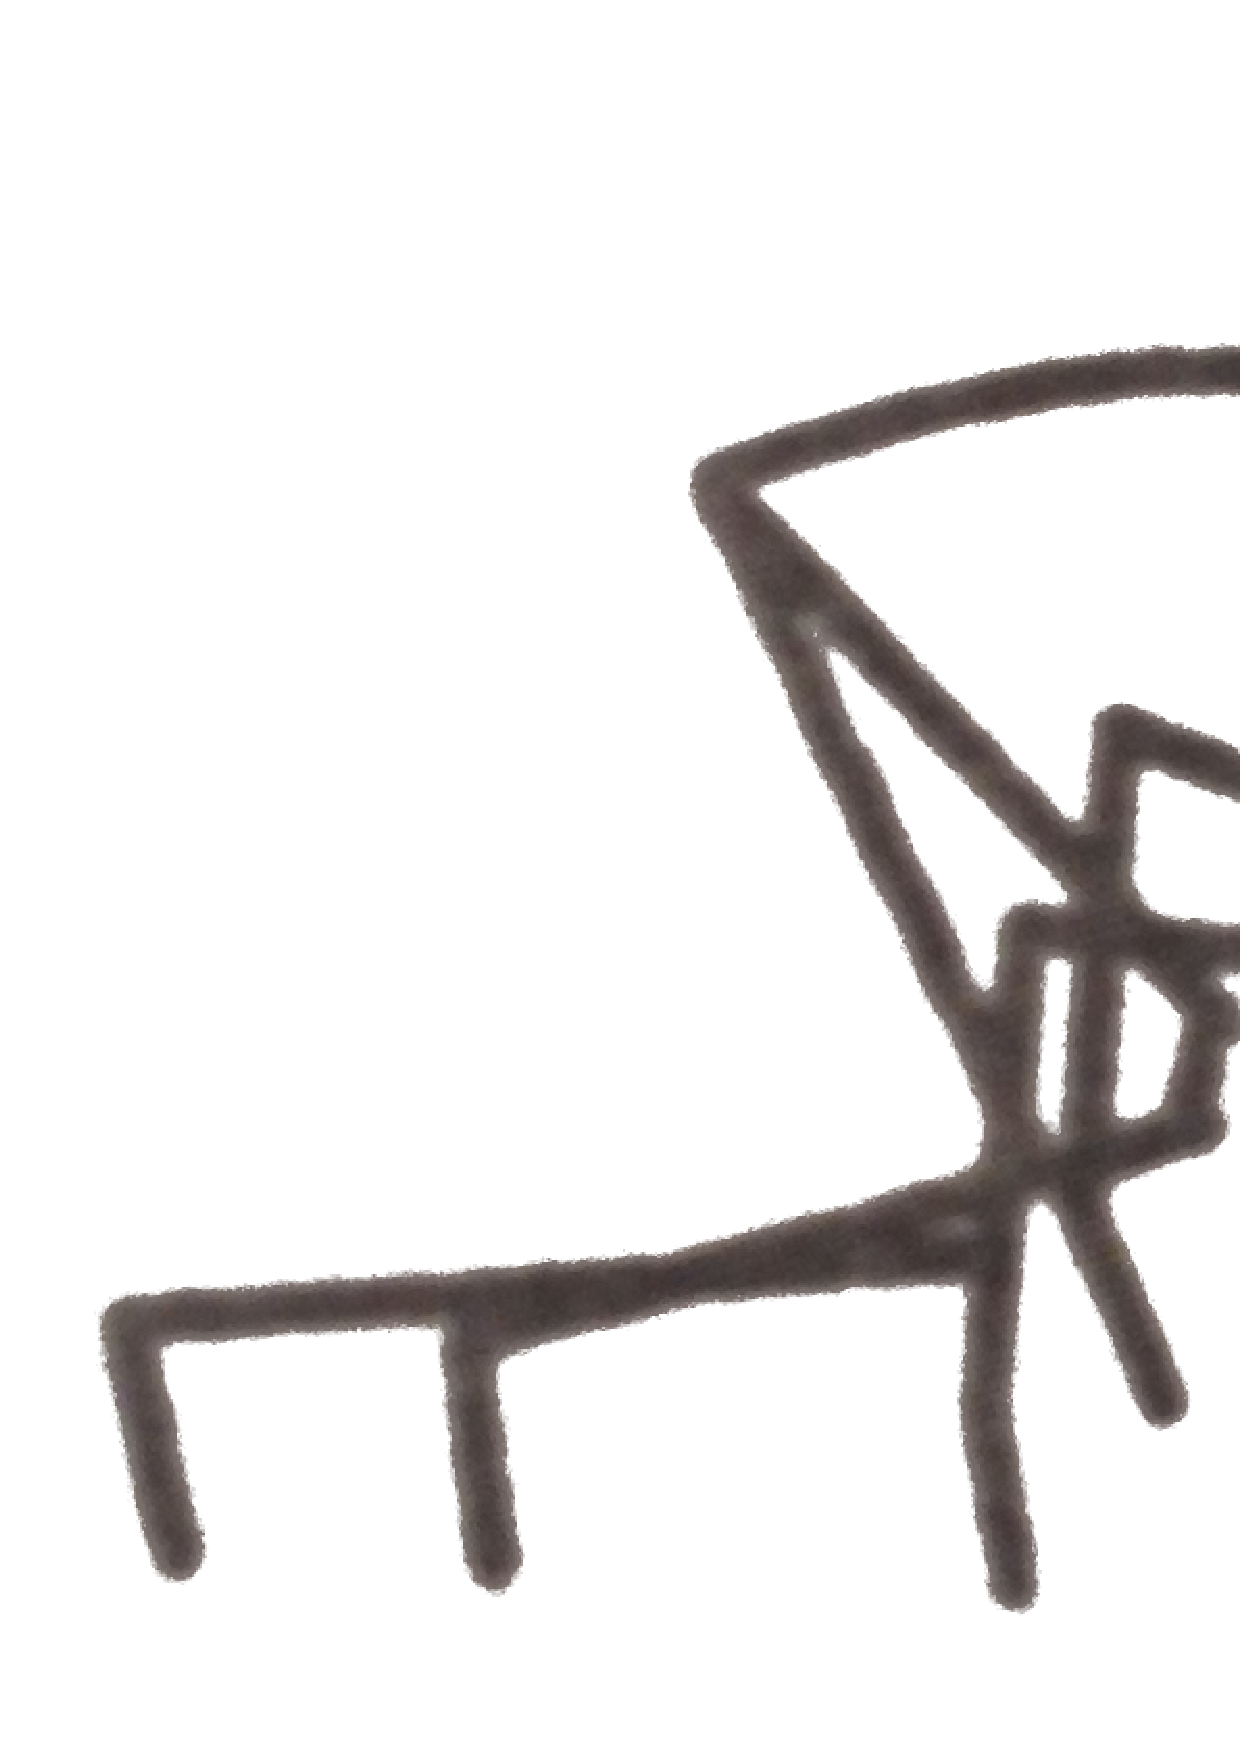
\includegraphics[width=1\linewidth]{HS_lift.png}
%	\end{figure}

	\column{0.4\textwidth} % Left column and width
\structure{Lift your knees} a bit off the ground. The pressure on the crown increases.

Try again in this position to \structure{roll} a bit forward and backwards. This will be way more difficult.                                                                                                                                                                                                                                                                                                                                                                                                                                                                                                                                                                                                                                                                                                                                                                                                                                                                                                                                                                                                                                                                                                                                                                                                                                                                                                                                                                                                                                                                                                                                                                                                                                                                                                                                                                                                                                                                                                                                                                                                                                                                                                                                                                                                                                                                                                                                                                                                                                                                                                                                                                                                                                                                                                                                                                                                                                                                                                                                                                                                                                                                                                                                                                                                                                                                                                                                                                                                                                                                                                                                                                                                                                                                                                                                                                                                                                                                                                                                                                                                                                                                                                                                                                                                                                                                                                                                                                                                                                                                                                                                                                                                                                                                                                                                                                                                                                                                                                                                                                                                                                                                                                                                                                                                                                                                                                                                                                                                                                                                                                                                                                                                                                                                                                                                                                                                                                                                                                                                                                                                                                                                                                                                                                                                                                                                                                                                                                                                                                                                                                                                                                                                                                                                                                                                                                                                                                                                                                                                                                                                                                                                                                                                                                                                                                                                                                                                                                                                                                                                                                                                                                                                                                                                                                                                                                                                                                                                                                                                                                                                                                                                                                                                                                                                                                                            
\end{columns}
\end{frame}
%---------------------------------------------------------------------------------
%-------------------------------------------------------------------
\begin{frame}
\frametitle{Lifting your legs}
\hypertarget{hemi}{}
\begin{columns}[c] % The "c" option specifies centered vertical alignment while the "t" option is used for top vertical alignment

\column{0.67\textwidth} % Left column and width
%	\begin{figure}
	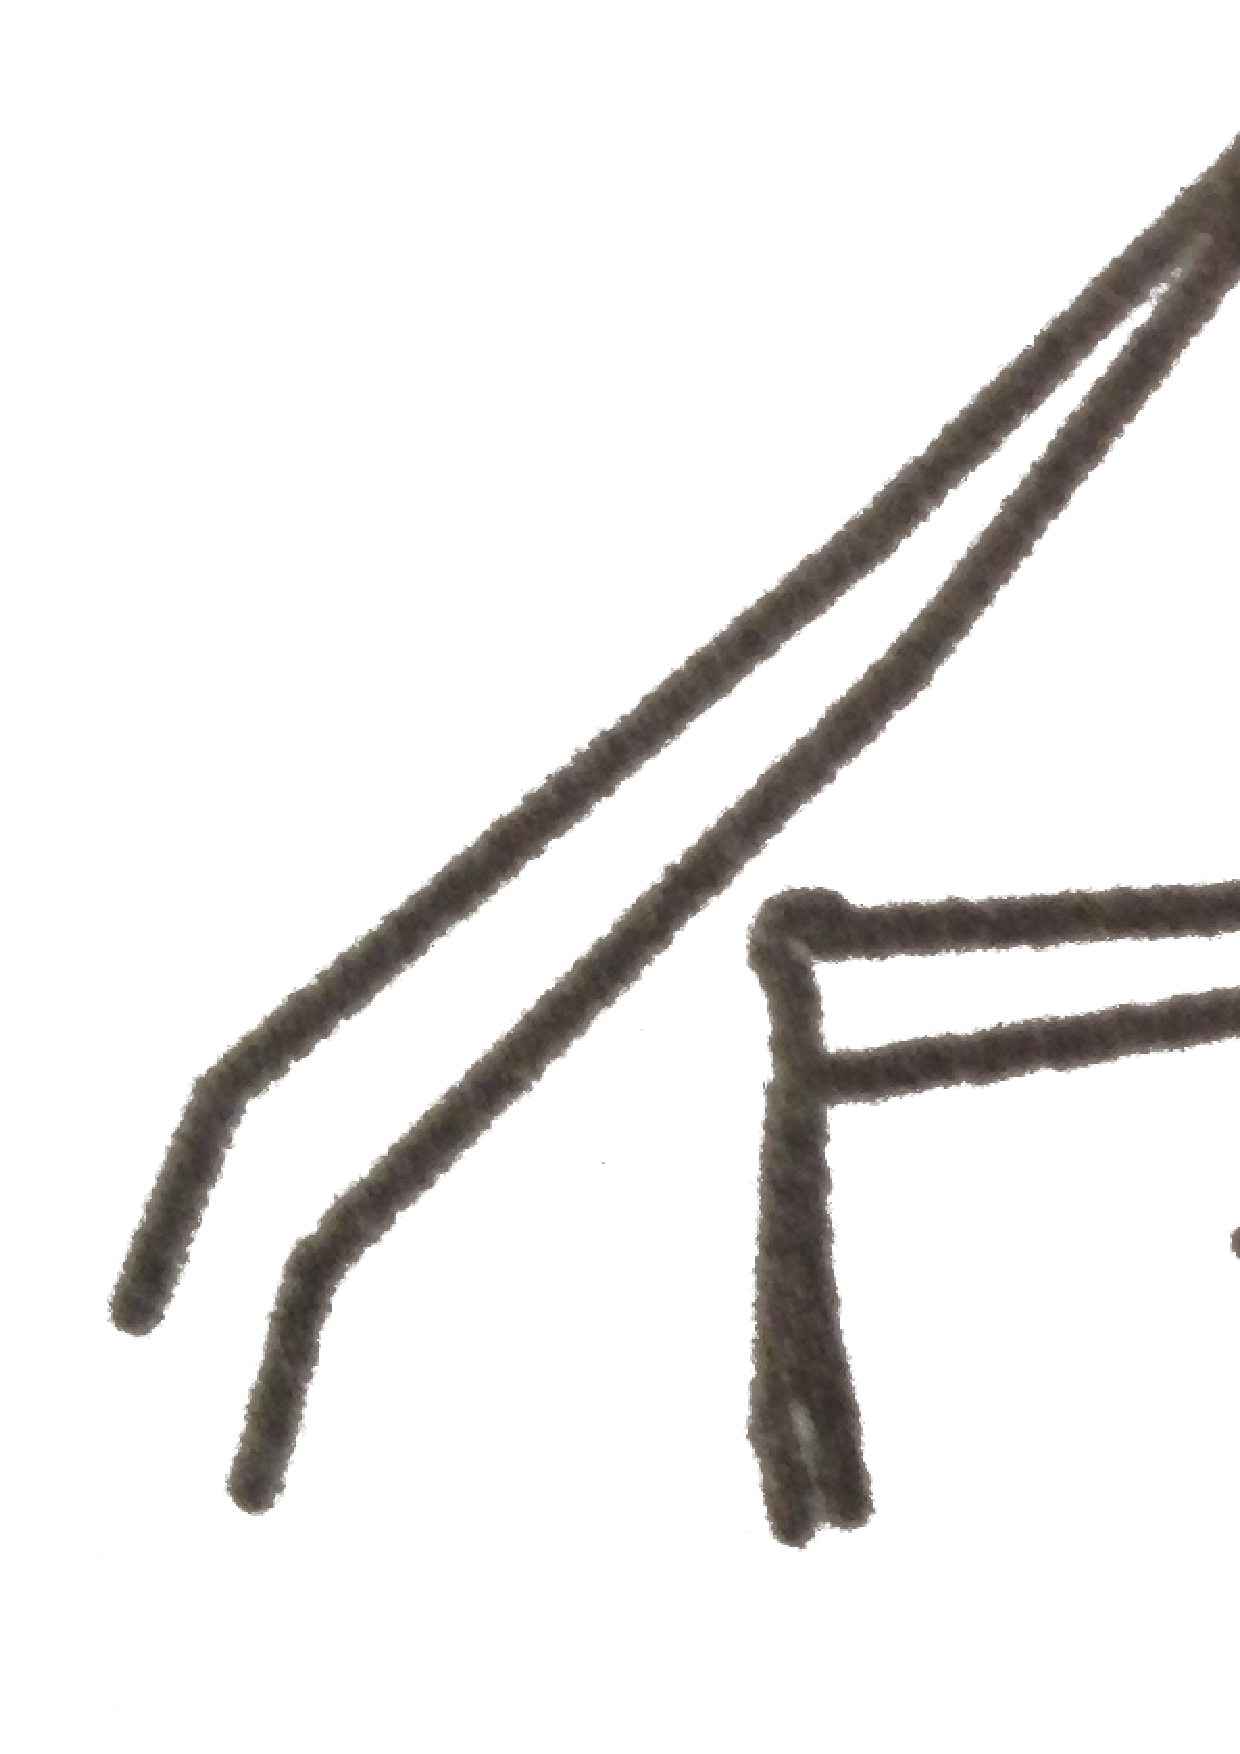
\includegraphics[width=1\linewidth]{HS_Upwards.png}
%	\end{figure}

	\column{0.33\textwidth} % Left column and width
\structure{Walk} with your \structure{feet} closer towards your head and push your \structure{backside towards ceiling}.

Try to bring your feet away from the ground by making a hollow back.

It's important to \structure{first bring the feet up}, not the  legs.                                                                                                                                                                                                                                                                                                                                                                                                                                                                                                                                                                                                                                                                                                                                                                                                                                                                                                                                                                                                                                                                                                                                                                                                                                                                                                                                                                                                                                                                                                                                                                                                                                                                                                                                                                                                                                                                                                                                                                                                                                                                                                                                                                                                                                                                                                                                                                                                                                                                                                                                                                                                                                                                                                                                                                                                                                                                                                                                                                                                                                                                                                                                                                                                                                                                                                                                                                                                                                                                                                                                                                                                                                                                                                                                                                                                                                                                                                                                                                                                                                                                                                                                                                                                                                                                                                                                                                                                                                                                                                                                                                                                                                                                                                                                                                                                                                                                                                                                                                                                                                                                                                                                                                                                                                                                                                                                                                                                                                                                                                                                                                                                                                                                                                                                                                                                                                                                                                                                                                                                                                                                                                                                                                                                                                                                                                                                                                                                                                                                                                                                                                                                                                                                                                                                                                                                                                                                                                                                                                                                                                                                                                                                                                                                                                                                                                                                                                                                                                                                                                                                                                                                                                                                                                                                                                                                                                                                                                                                                                                                                                                                                                                                                                                                                                                       
\end{columns}
\end{frame}
%---------------------------------------------------------------------------------
%-------------------------------------------------------------------
\begin{frame}
\frametitle{Legs up}
\hypertarget{hemi}{}
\begin{columns}[c] % The "c" option specifies centered vertical alignment while the "t" option is used for top vertical alignment

\column{0.33\textwidth} % Left column and width
%	\begin{figure}
	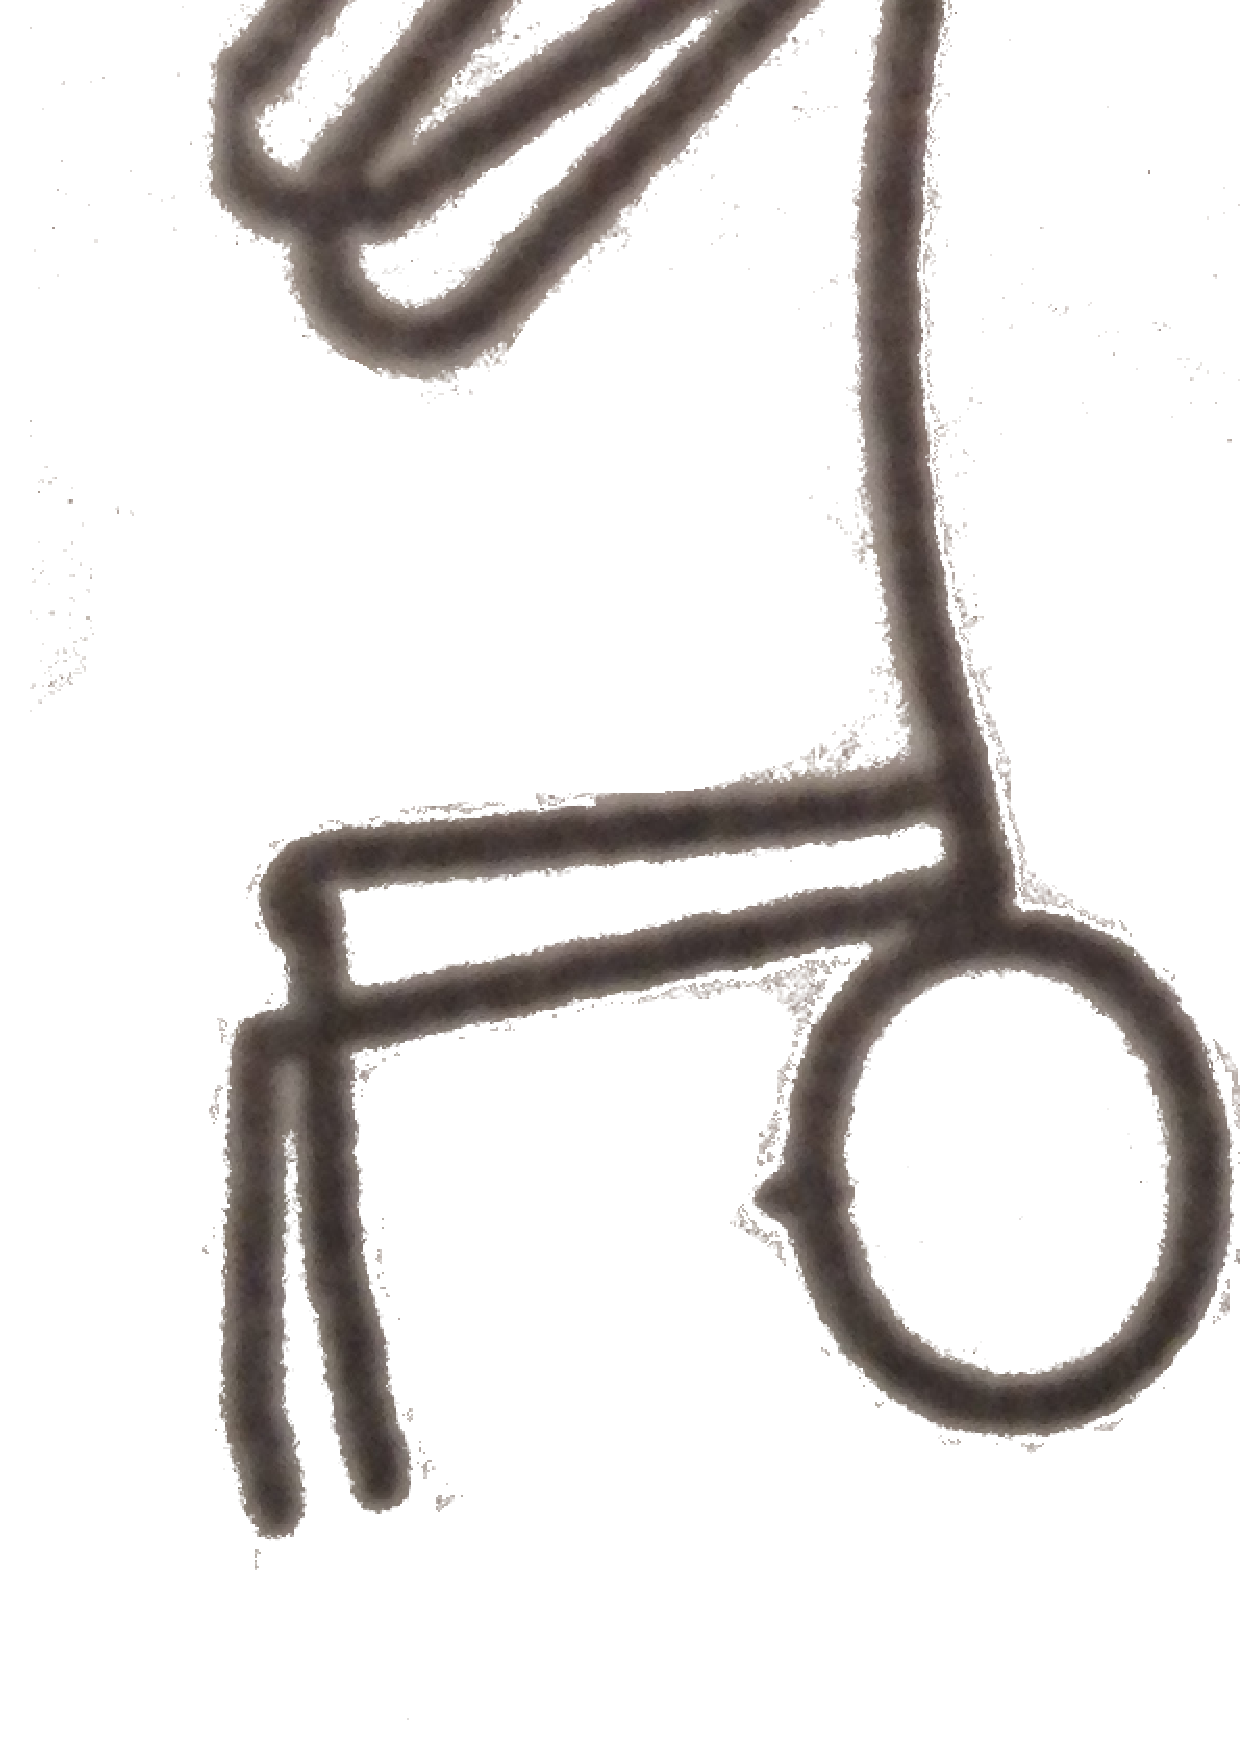
\includegraphics[width=1\linewidth]{HS_Up.png}
%	\end{figure}

	\column{0.5\textwidth} % Left column and width
Now pull your \structure{legs slowly up} with your hips. 

Let them \structure{first be tucked in} and only then \structure{slowly up} when you feel safe to do so.                                                                                                                                                                                                                                                                                                                                                                                                                                                                                                                                                                                                                                                                                                                                                                                                                                                                                                                                                                                                                                                                                                                                                                                                                                                                                                                                                                                                                                                                                                                                                                                                                                                                                                                                                                                                                                                                                                                                                                                                                                                                                                                                                                                                                                                                                                                                                                                                                                                                                                                                                                                                                                                                                                                                                                                                                                                                                                                                                                                                                                                                                                                                                                                                                                                                                                                                                                                                                                                                                                                                                                                                                                                                                                                                                                                                                                                                                                                                                                                                                                                                                                                                                                                                                                                                                                                                                                                                                                                                                                                                                                                                                                                                                                                                                                                                                                                                                                                                                                                                                                                                                                                                                                                                                                                                                                                                                                                                                                                                                                                                                                                                                                                                                                                                                                                                                                                                                                                                                                                                                                                                                                                                                                                                                                                                                                                                                                                                                                                                                                                                                                                                                                                                                                                                                                                                                                                                                                                                                                                                                                                                                                                                                                                                                                                                                                                                                                                                                                                                                                                                                                                                                                                                                                                                                                                                                                                                                                                                                                                                                                                                                                                                                                                                                                                   
\end{columns}

\vspace{1cm}
Back to \href{run:./Exercises.pdf}{\underline{exercises}}.
\end{frame}
%---------------------------------------------------------------------------------


\end{document} 